\documentclass[12pt]{article}
\usepackage[italian]{babel}
\usepackage[utf8x]{inputenc}
\usepackage{amsmath}
\usepackage{graphicx}
\usepackage{hyperref}
\usepackage{eurosym}

\begin{document}
	\begin{titlepage}
			\newcommand{\HRule}{\rule{\linewidth}{0.5mm}} % Defines a new command for the horizontal lines, change thickness here
		
		\center % Center everything on the page
		
		%----------------------------------------------------------------------------------------
		%	HEADING SECTIONS
		%----------------------------------------------------------------------------------------
		
		\textsc{\LARGE Università degli studi di Padova}\\[1.5cm] % Name of your university/college
		
\includegraphics[scale=0.3]{images/unipd_logo.png}\\[1cm] % Include a department/university logo - this will require the graphicx package
		\textsc{\Large Relazione progetto per il corso di Web Information Management}\\[0.5cm] % Major heading such as course name
		\textsc{\large Corso di Laurea in Informatica, A.A. 2016-2017}\\[0.5cm] % Minor heading such as course title
		%----------------------------------------------------------------------------------------
		%	TITLE SECTION
		%----------------------------------------------------------------------------------------
		
		\HRule \\[0.4cm]
		{ \huge \bfseries Analisi usabilità strumentimusicali.net}\\[0.4cm] % Title of your document
		\HRule \\[1.5cm]
		
		%----------------------------------------------------------------------------------------
		%	AUTHOR SECTION
		%----------------------------------------------------------------------------------------
			\begin{minipage}{0.4\textwidth}
				\begin{flushleft} \large
					\emph{Studente:}\\
				 Matteo Slanzi \\ \#1100866
				\end{flushleft}
			\end{minipage}
			~
			\begin{minipage}{0.4\textwidth}
				\begin{flushright} \large
					\emph{Docente:} \\
					Massimo Marchiori
				\end{flushright}
			\end{minipage}\\[2cm]
		
		
		\vfill % Fill the rest of the page with whitespace
	\end{titlepage}
	\newpage
	\renewcommand{\contentsname}{Indice}
	\tableofcontents
	\newpage
	\listoffigures
	\newpage
	\section{Introduzione}
	\vspace {0.5cm}
	\textbf{Link al sito: }    \url{http://www.strumentimusicali.net/} \\
	\\
	Il progetto riguardante il corso di Web Information Management consiste nell'analisi di usabilità di un sito web.\\ La mia scelta riguarda un sito di e-commerce di strumenti musicali che vende, principalmente in Italia, una vasta gamma di strumenti e accessori musicali, sia professionali che amatoriali. 
	\\
	Il sito mi è sembrato fin da subito ben fatto e ho deciso di analizzarlo, anche per via di un acquisto di un paio di cuffie fatto qualche mese fa.
	\newpage
	\section{Analisi delle pagine}
		\subsection{Homepage}
	La homepage del sito è molto ricca, nell'header troviamo subito il logo del sito, il menu, la barra di ricerca e lo slideshow che mostra gli articoli in sconto o novità. Più sotto troviamo gli articoli in evidenza, gli ultmi arrivi del mese, ultime recensioni e news. In fondo, il footer raggruppa diverse informazioni quali, l'assistenza post vendita, le modalità di pagamento e consegna, diritti e privacy, link ai vari social e tutte le informazione dell'azienda che si occupa della gestione e vendita dei prodotti del sito.
	\vspace{1cm}
	\begin{figure}[ht!]
		\centering	
		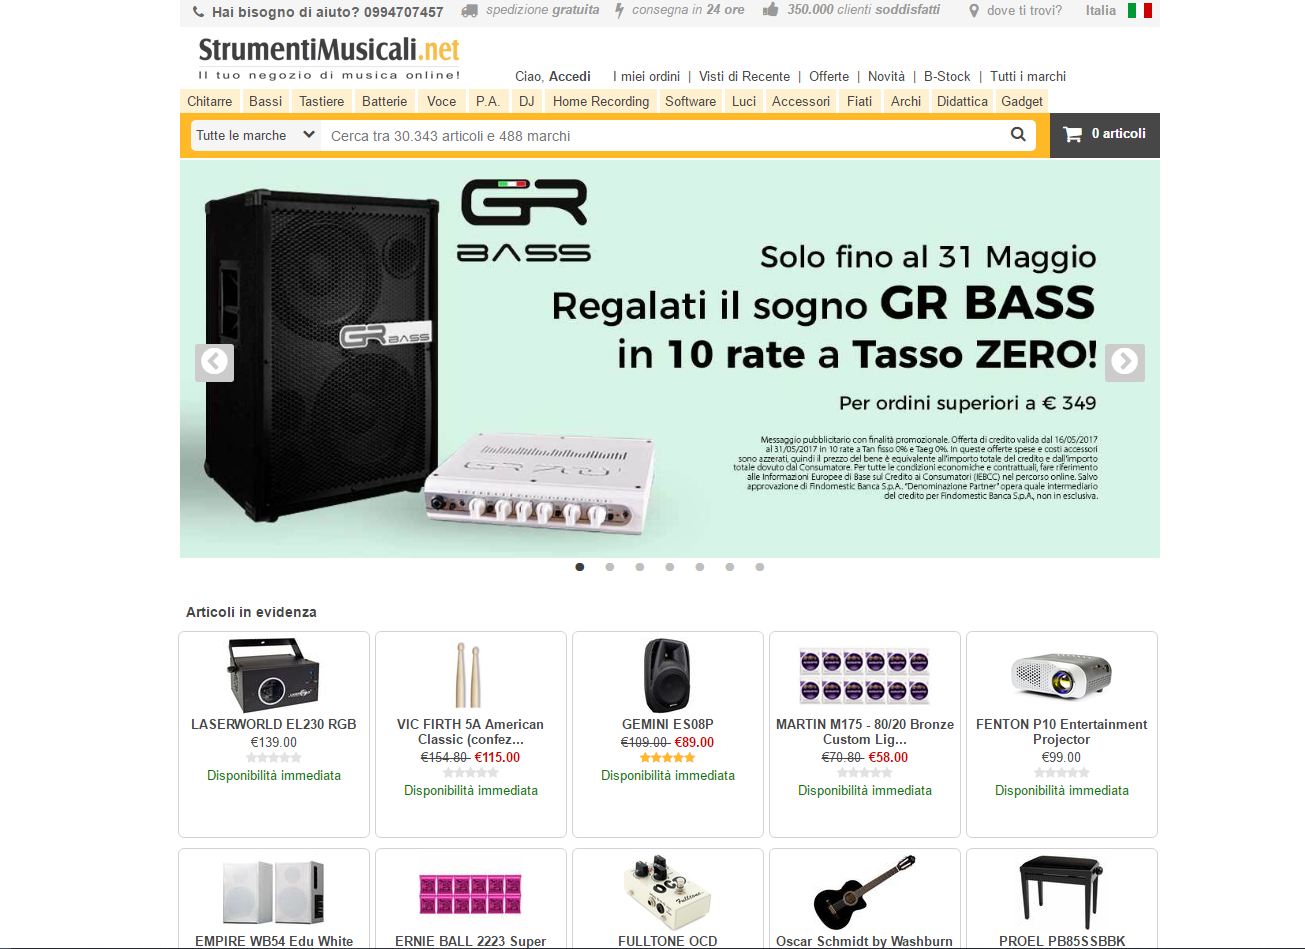
\includegraphics[width=150mm]{images/home.png}
		\caption{Homepage scroll 1}
	\end{figure}
	\begin{figure}
		\centering	
		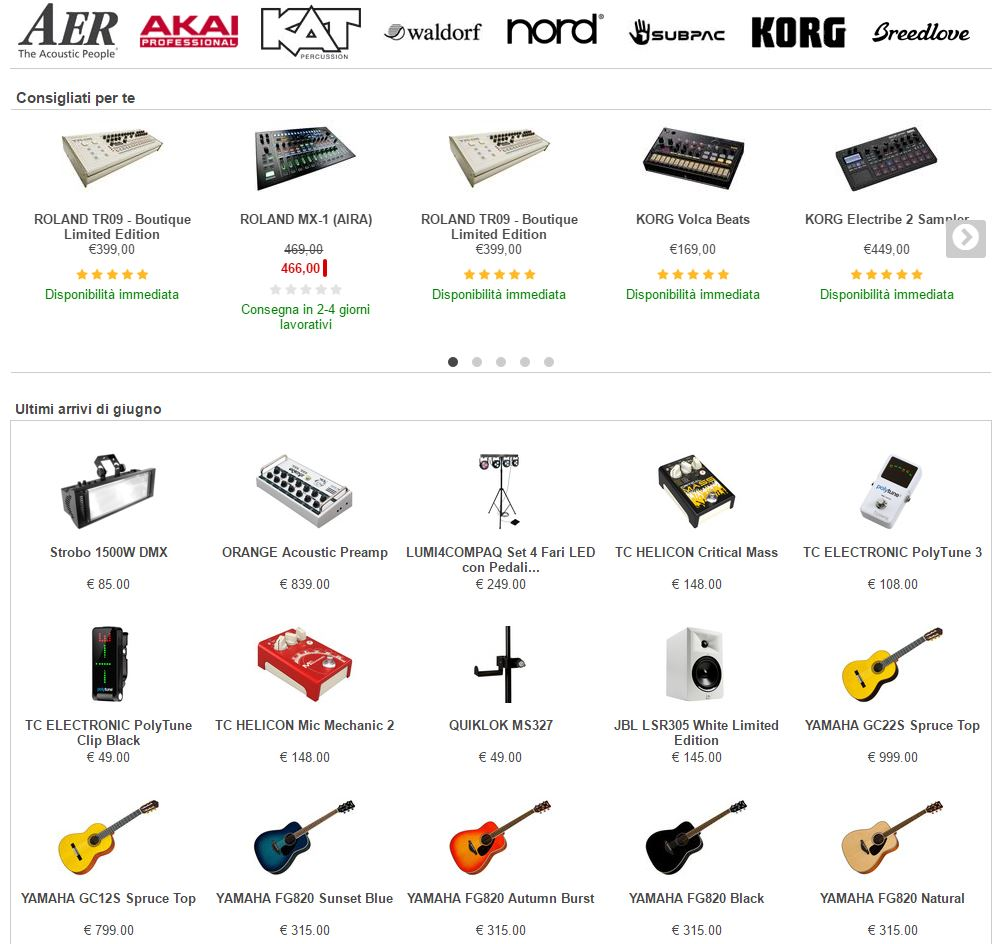
\includegraphics[width=160mm]{images/home2.png}%
		\caption{Homepage scroll 2}
	\end{figure}
	\begin{figure}
		\centering	
		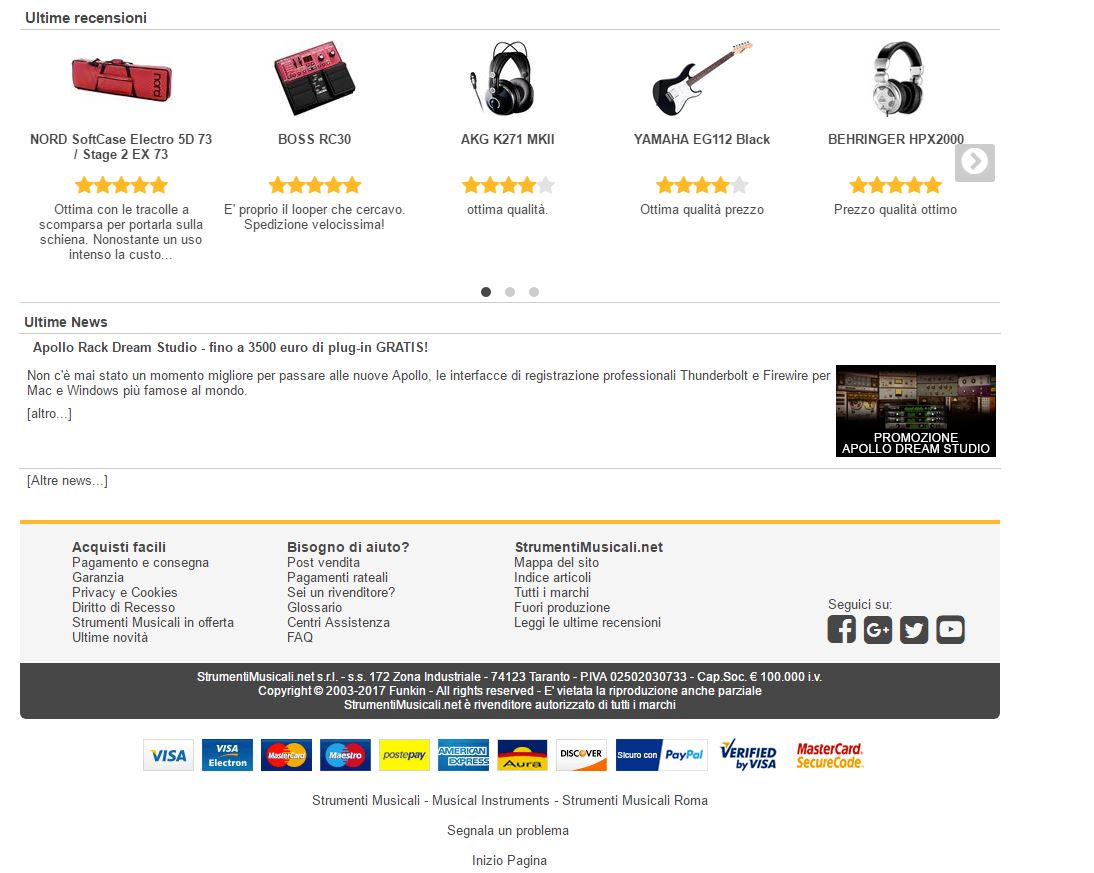
\includegraphics[width=160mm]{images/home3.png}%
		\caption{Homepage scroll 3}
	\end{figure}
	\newpage
	\subsection{Assi fondamentali}
	\vspace{0.5cm}
	Per prima cosa cerco di analizzare la pagina e provo a immedesimarmi nell'utente che visita per la prima volta il sito. Riesce a capire in che sito è finito? E trova quello che stava cercando?  Queste e altre domande fanno parte delle 6W che caratterizzano gli assi fondamentali di una pagina web.
	\paragraph{1) Where} "Dove mi trovo? In che sito sono arrivato? "
	\\ 
	A prima vista si nota subito che è un sito di strumenti e accessori musicali, lo slideshow in primo piano mostra diversi prodotti musicali, come casse audio e chitarre. Non è difficile capire che è un sito che vende strumenti musicali, nel logo notiamo la scritta "Il tuo negozio di musica online", inoltre possiamo vedere gli articoli in evidenza che presentano prezzo e disponiblità.
	\paragraph{2) What} "Cosa offre il sito? Cosa posso trovare? "
	\\
	L'indice del sito lo possiamo trovare in alto sotto il logo del sito. L'indice mostra le varie categorie di prodotti che offre, come chitarre, bassi, software e accessori.. \\ Nello slideshow vengono mostrati vari articoli, come novità o prodotti in notevole sconto, se clicchiamo nello slideshow verremo reindirizzati alla pagina del prodotto. 
	\paragraph{3) Who} "Chi rappresenta il sito? "
	\\
	In alto a sinistra possiamo notare il logo del sito dell'azienda, punto importante per l'utente che permette di identificare il nome del sito. Se clicco sopra il logo ho solamente un refresh della home. Le informazioni dell'azienda le possiamo trovare nel footer dopo diversi scroll. 
	\paragraph{4) Why} "Perchè dovrei fermarmi su questo sito? Quali benefici mi porta?"
	\\
	Il perchè dovrei acquistare su questo sito non è visibile, però facendo un confronto dei prezzi che possiamo trovare in altri siti web o negozi fisici, si nota che ha dei prezzi pari o inferiori su quasi tutti i prodotti, risparmiando così diversi soldi. Inoltre è un sito specializzato con una vasta gamma di prodotti che difficilmente si può trovare in altri negozi.
	\newpage
	\paragraph{5) When} "Quali sono le novità del sito? "
	\\
	Le novità del sito le possiamo trovare sopra il menù nella sezione "Novità", cliccandoci sopra verremo reindirizzati alla pagina interna di tutti i nuovi articoli inseriti nel sito. Possiamo filtrare gli articoli in base alla categoria che ci interessa e ordinarli per prezzo crescente/decrescente o in ordine alfabetico. \\
	I nuovi arrivi li possiamo trovare anche nello slideshow, magari con una promozione e più sotto dopo un paio di scroll è presente la sezione degli ultimi arrivi del mese.
	\paragraph{6) How} "Come navigo nel sito? Come arrivo a quello che mi interessa? "
	\\
	Per navigare nel sito possiamo usare il menu per accedere alle varie categorie, è menu di tipo hover e se ci passo sopra con il mouse si apre una tendina con le varie sottocategorie. Il menu a tendina uscendo dal riquadro sparisce costrigendomi a riaprire la categoria scelta. A mio parere si sarebbe potuto lasciare un lasso di tempo di qualche secondo in cui rimaneva aperto il menu a tendina. Per quanto riguarda il testo si sarebbe potuto optare per una dimensione leggermente maggiore rendendolo così più leggibile.  \\
	E' presente anche una barra di ricerca, ben riconoscibile dall'utente per via della lente (la metafora visiva viene quindi rispettata), che ci permette di trovare un qualsiasi prodotto. Il box di ricerca è molto grande e supera abbondantemente i 50 caratteri, accontentando così la maggior parte delle richieste degli utenti che possono scrivere una query più lunga e avere risultati più specifici.  Se la barra di ricerca è troppo piccola si ha lo scroll sul box e questo stressa gli utenti, inoltre induce l'utente a scrivere query più corte e meno specifiche ottenendo risultati più generici.
	\newpage
	\paragraph{Considerazioni}
	Lo stile della homepage è semplice e pulito, non vengono utilizzati colori sgargianti e il contrasto tra gli elementi della pagina e lo sfondo è ben visibile senza creare difficoltà nella lettura.
	Lungo tutta la pagina sono presenti varie sezioni quali gli articoli in evidenza, i prodotti consigliati per te, gli ultimi arrivi del mese etc. 
	\\
	Lo slideshow è ben fatto, mostra vari prodotti come novità o promozioni, resta fisso e per spostarci nelle varie immagini possiamo usare le frecce a destra e sinistra oppure i puntini di selezione sotto. Sarebbe stato opportuno avere dei puntini di selezione più grandi rendendo più facile la selezione, infatti per la legge di Fitts gli oggetti più grandi sono più facili da raggiungere e cliccare.\\ Le informazioni mostrate nello sldieshow non sono molto complete e a volte costringono l'utente a fare gambling click per vedere ulteriori informazioni.\\
	La lunghezza della pagina è abbastanza elevata costringendo l'utente a fare diversi scroll per arrivare in fondo alla pagina e trovare le informazioni che cercava. Sappiamo che l'utente nel web è pigro e la maggior parte degli utenti è disposta a fare scroll per 1.3 schermi, quindi 2.3 schermi totali e di conseguenza buona parte della pagina non verrà visualizzata. 
	\newpage
	\section{Pagine interne}
	Se andiamo sulla sezione delle chitarre classiche avremo una vasta gamma di modelli di chitarre, da quelle più economiche a quelle più costose. \\ A sinistra troviamo il riquadro con le varie sottocategorie delle chitarre, più sotto troviamo le chiatarre classiche più vendute, le ultime recensioni e ancora più sotto una sezione dove poter trovare un'idea regalo scegliendo un prezzo minimo e massimo. \\ A destra possiamo trovare le sezioni per filtrare per marca e disponibilità le chitarre, aiutando così l'utente a trovare più agevolmente il modello di chitarra che più lo soddisfa.
	\begin{figure}[ht!]
		\centering	
		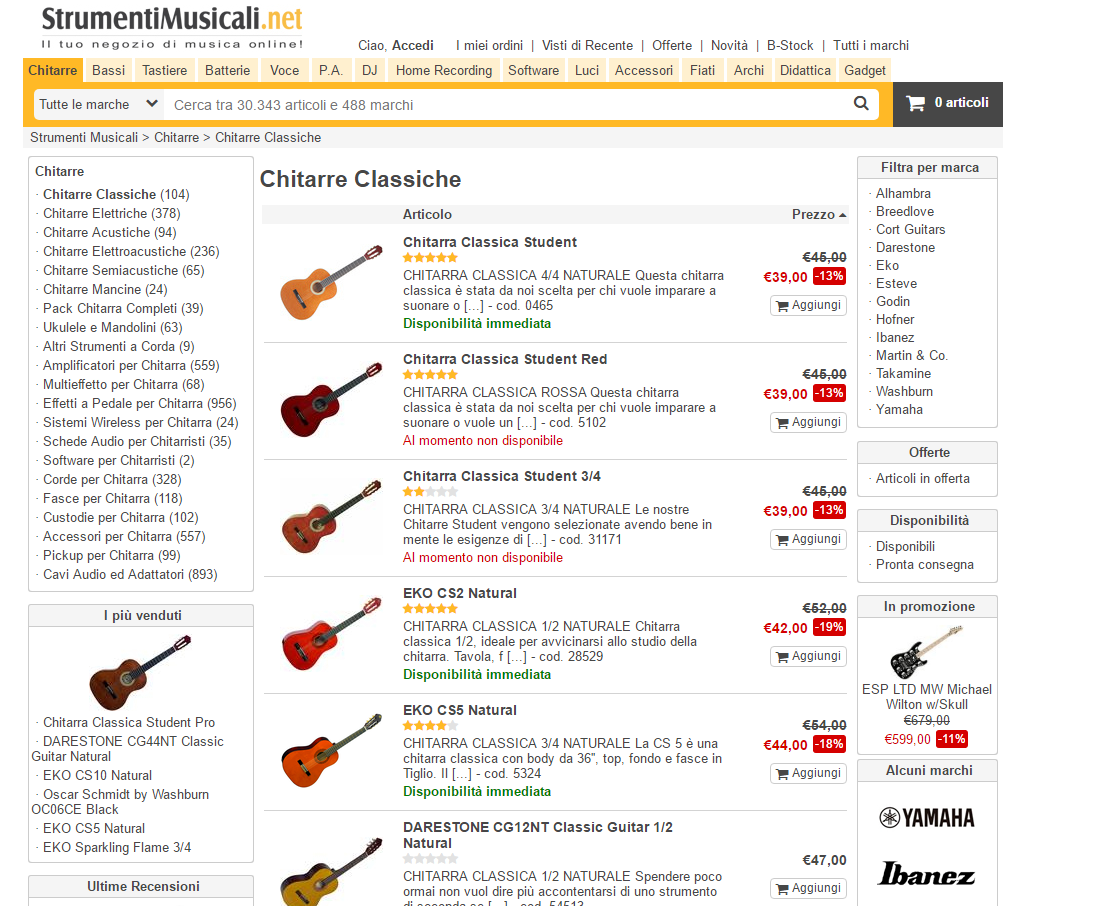
\includegraphics[width=130mm]{images/paginaInterna.png}
		\caption{Pagina interna delle chitarre classiche - \url{www.strumentimusicali.net/default.php/cPath/21_22/Chitarre/Chitarre-Classiche.html}}  
	\end{figure}
	\newpage
	\subsection{Assi obbligatori}
	\vspace{0.5cm}
	Alcuni assi per garantire una buona usabilità devono essere obbligatori su tutte le pagine del sito:
	\paragraph{Where} In ogni pagina l'asse where dovrebbe essere sempre presente, in modo da non creare confusione all'utente e sapere sempre dove si trova, infatti con il fenomeno del deep linking l'utente arriva tramite la ricerca direttamente a una pagina interna, evitando quindi di passare dalla homepage. Per fare questo il sito strumentimusicali.net utilizza un breadcrumb di tipo Location, mostrando il percorso intero fino alla pagina corrente. 
	\paragraph{What} L'asse what rimane invariato, è sempre presente in ogni pagina interna il menu con tutte le varie categorie di prodotti.
	\paragraph{Who} In alto a sinistra troviamo sempre il logo del sito che cliccandoci sopra ci riporta alla homepage.
	\\
	\subsection{Assi opzionali consigliati}
	\vspace{0.5cm}
	\paragraph{How} Come arrivare ad altre sezioni del sito non cambia, il layout rimane lo stesso e possiamo spostarci su altre categorie tramite il menu in alto.
	\paragraph{Why} Non ci sono descrizioni sul perchè dovremo acquistare su questo sito, però nelle varie pagine interne di ogni sottocategoria notiamo che alcuni articoli sono scontati e hanno prezzi più competitivi rispetto ad altri negozi.
	\paragraph{When} Le novità e gli ultimi arrivi li possiamo sempre trovare nell'apposita sezione sopra il menu.
	\newpage
	\subsection{Pagina singolo articolo}
	\vspace{0.4cm}
	Nella pagina del singolo articolo troviamo il titolo del modello, sotto è presente il rating del prodotto fatto con le recensioni dei clienti che lo hanno acquistato, in questo modo l'utente si fa un'idea sulla qualità dell'articolo. Cliccando sopra la valutazione veniamo rimandati alle recensioni complete del prodotto.
	\\ E' presente una grande immagine del prodotto che rispetta quindi le dimensioni minime, è presente anche uno strumento di zoom passando sopra col mouse sull'immagine, mentre se clicchiamo l'immagine si apre la pagina con dimensioni maggiori per visualizzarla nel dettaglio. Alcuni articoli hanno una sola immagine mentre altri sono accompagnati da diverse immagini che mostrano nel dettaglio da più prospettive il prodotto. \\
	 A destra la sezione delle informazioni di vendita del prodotto è ben fatta, il prezzo è ben visibile e viene mostrata la percentuale di sconto e il risparmio in \euro, viene riportata la disponibilità e la quantità che vogliamo acquistare. E' presente anche un bottone per le informazioni sulle spese di spedizioni che cliccandoci sopra ci apre un pop-up con le relative informazioni. La scelta del pop-up poteva essere evitata in quanto gli utenti non la gradiscono molto e cercano subito come chiuderla. \\
	 Sotto l'immagine abbiamo una descrizione del prodotto e alcune caratteristiche principali. In altre pagine di prodotti più tecnici ed elettronici possiamo trovare una ricca scheda tecnica e anche un file pdf con tutte le caratteristiche del prodotto, in questo modo l'utente può conoscere perfettamente nel dettaglio il prodotto che sta cercando. \\ Più in basso troviamo una sezione dei prodotti che potrebbero servirci per l'articolo che stiamo guardando, aiutandoci così a trovare immediatamente eventuali accessori da abbinare con l'articolo.
	 \begin{figure}
	 	\centering	
	 	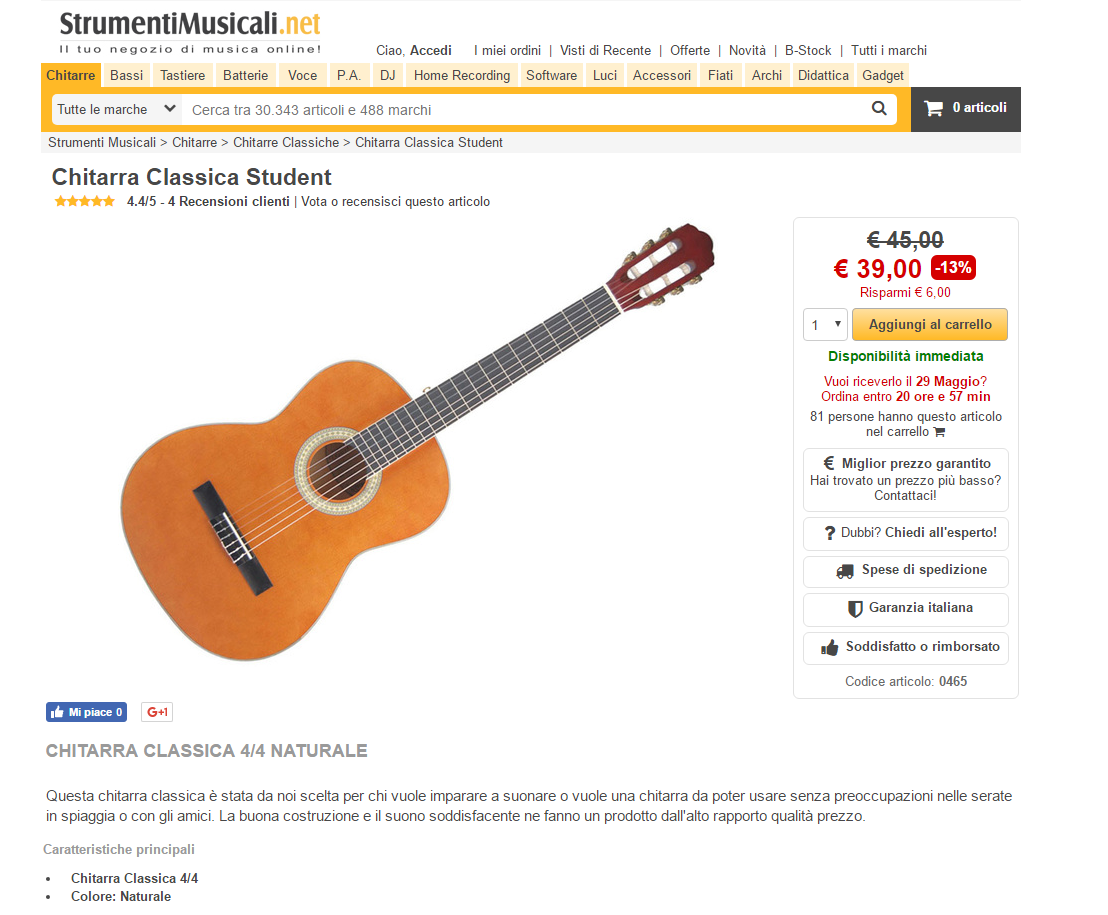
\includegraphics[width=180mm]{images/paginaProdotto.png}
	 	\caption{Pagina interna di una chitarra classica - \url{www.strumentimusicali.net/product_info.php/cPath/21_22/products_id/465/chitarra-classica-student.html}} 
	 \end{figure}
 	\newpage
	\subsection{Pagina carrello}
	\vspace{0.4cm}
	La pagina carrello ci mostra la lista degli articoli pronti per essere acquistati, è presente l'immagine del prodotto con la quantità e il prezzo. Possiamo rimuovere facilmente un prodotto con la X tra il codice e il prezzo, mentre se si vuole aggiungere o diminuire la quantità di un articolo basta premere sui bottoni + e - della quantità.
	\\ Il totale dell'ordine è ben visibile ed ulteriori spese sono riportate, come per esempio chi acquista con contrassegno dovrà pagare 5.90 \euro in più, mentre le altre modalità di pagamento non hanno ulteriori costi. \\Viene mostrata una sezione sui servizi offerti e il loro relativo costo, in questo caso l'imballaggio rinforzato, la spedizione assicurata e la notifica SMS sono gratis. Per quanto riguarda i costi di spedizione sono gratuiti per gli ordini sopra i 199\euro, in questo caso con un totale di 202\euro la consegna tramite corriere espresso è gratuita. 
	\\ Per quanto riguarda i tempi di consegna non sono molto chiari al momento del checkout, ma viene comunque inserito un intervallo di pochi giorni in cui avviene la consegna.
	\begin{figure}
		\centering	
		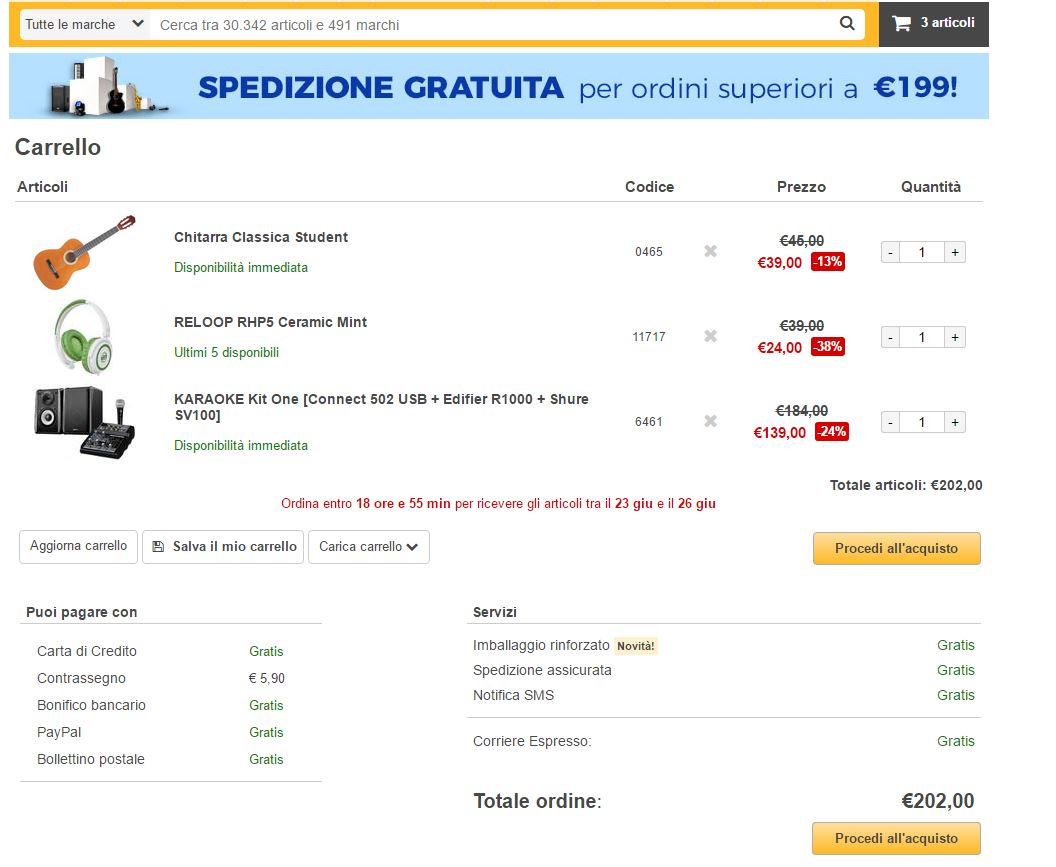
\includegraphics[width=180mm]{images/carrello.png}
		\caption{Pagina del carrello -  \url{www.strumentimusicali.net/shopping_cart.php}}
	\end{figure}
	\newpage
	\subsection{Pagina 404}
	\vspace{0.5cm}
	Se provo ad accedere ad una pagina inesistente, il sito riporta correttamente il messaggio che la pagina non è stata trovata, il link alla homepage sul logo funziona correttamente. Una  pagina generica con scritto: "Error 404" può far perdere diversi possibili clienti.
	\begin{figure}[ht!]
		\centering	
		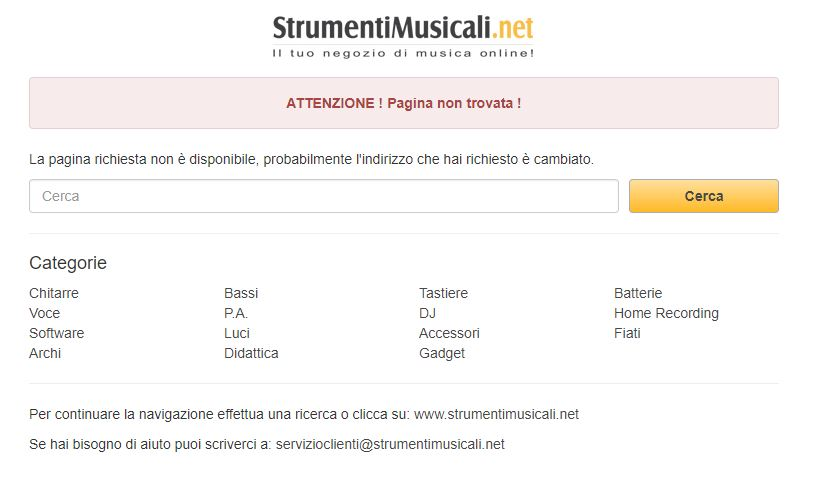
\includegraphics[width=180mm]{images/404.jpg}
		\caption{Pagina non trovata}
	\end{figure}
	\newpage
	\section{Considerazioni generali}
	\vspace{0.5cm}
	\paragraph{Design} Lo stile grafico adottato è semplice e chiaro, vengono usati colori neutri e pochi carichi come bianco, nero e tonalità di grigio, non vengono usati colori particolarmente vivaci se non nello slideshow per mettere in evidenza determinati articoli. Non sono presenti testi lampeggianti, molto fastidiosi all'utente e neppure elementi di bloated design che comportano un'elevata difficoltà computazionale all'utente. \\
	Non è presente nessuna pagina splash di benvenuto che sostituisce la homepage, sono da evitare a tutti i costi in quanto fanno solo perdere tempo all'utente. 
	\\
	\paragraph{Testo} Il testo in tutto il sito è ben visibile grazie all'ottimo contrasto tra colore nero del testo e sfondo bianco e con dimensioni del font adeguate. Nel menu il contrasto rimane buono anche su sfondo giallo chiaro, mentre la dimensione del font usato risulta leggermente piccola e visto che non è presente nessun resize del testo,  gli utenti con difficoltà nella lettura non vengono agevolati. 
	\\Non viene usato testo come elemento grafico della pagina e il font è chiaro e leggebile ed è lo stesso su tutto il sito.
	\\
	\paragraph{Finestre e Pop-up} L'apertura dei vari link alle pagine interne, ai link del menu e delle immagini non comporta mai l'apertura di una nuova scheda o finestra. Questa scelta è molto apprezzata dagli utenti in quanto la navigazione non diventa dispersiva e la funzione di back button permette di non spostare il flusso di navigazione.
	\\
	\newpage
	\paragraph{Pubblicità} Non è presente alcuna pubblicità nel sito, è un negozio online e non offrendo un servizio gratutito per gli utenti non ha bisogno di pubblicità. La sua fonte di reddito deriva esclusivamente dalla vendita dei prodotti che offre, quindi potremmo trovare la pubblicità di questo negozio in altri siti che offrono contenuti gratuiti agli utenti. 
	\\
	\paragraph{Registrazione} Per poter acquistare i prodotti, come in ogni negozio online, serve la registrazione. Il sito comunque rimane completamente navigabile anche senza essere registrati e gli utenti possono consultare facilmente i dettagli tecnici dei prodotti e le eventuali recensioni.
	\\
	\paragraph{Descrizione e immagini degli articoli} La descrizione dei prodotti è sempre presente, un sito che non ha descrizioni viene ritenuto poco professionale e fa migrare l'utente in altri siti.\\
	In quasi tutti gli articoli sono presenti più immagini da diverse prospettive e disponibili in full-screen, fattore molto positivo in quanto l'utente, non potendolo vedere dal vivo, vuole vederlo in ogni dettaglio.
	\\    
	\paragraph{Prezzo dei prodotti} Il prezzo degli articoli è ben visibile fin da subito all'utente e non si ha nessun gambling click per scoprire il prezzo del prodotto. Il gambling click è da evitare in quanto l'utente deve cliccare col dubbio di fare qualcosa di giusto. Quando è presente il gambling click il gradimento del sito scende abbondantemente e i link vengono cliccati solamente il 30\% delle volte.
	\\ 	Non vengono usate tecniche di fishing price, ossia utilizzare un prezzo estremamente conveniente per attirare l'attenzione dell'utente. Il prezzo è compreso di tasse ed eventuali spese di spedizioni le troviamo in ogni singolo prodotto cliccando il buttone delle spese di spedizione oppure nella pagina di riepologo del carrello.
	\newpage
	\section{Valutazione}
	\vspace{0.5cm}
	Il sito non presenta criticità rilevanti e all'utente medio la navigazione risulta piacevole e non confusionaria. Il sito sicuramente è stato realizzato prestando attenzione ai comportamenti dell'utente medio nel web per favorire la permanenza e indurre l'utente a comprare in questo sito. 
	\\
	\\
	\textbf{Voto: 8.5}
	
\end{document}
